% This is the root file of your thesis: thesis.tex
% A line starting with % is a comment. In some cases, I have included a command preceded by a %. You may activate the command by removing the %.


%%===================================
\documentclass[10pt,table]{report}
\usepackage{GGstyle}
%%===================================
\usepackage{natbib}
\bibliographystyle{agsm}
\usepackage{url}
%%===================================
%Write the various parts of your thesis as separate files and include them into the main file by the command \include{name of included file}. When you compile the LaTeX file, you may choose which subfiles to include by the command

%\includeonly{chapter01,chapter02}
%AA------------------------------- TODO og referere til andre kapitler --------------------------------
\usepackage{todonotes} %To make todo-notes
\usepackage{xr} %Referere til kapitler i andre tex-dokumenter
%\usepackage[nonumberlist,toc]{glossaries}%Adding glossary, and adding it to contents. "nonumberlist" removes page reference in glossary

%\usepackage{biblatex}
%\addbibresource{bibtex/library.bib}

%AA------------------------------- Figure layout --------------------------------
\usepackage{graphicx} % To include images
\graphicspath{ {figures/} } %To add list of figures
\usepackage[font=footnotesize, labelfont=bf]{caption} %Setting size of figure text, and making figure numbering bold
\captionsetup{width=0.9\linewidth} %Setting global width of figure text (can also be set specifically for one figure)
\usepackage{caption}
\usepackage{subcaption} %To add caption for each independend side-by-side figure

\usepackage{float}%To allow [H] after figures/tables ++ to force placement


%%===================================
\begin{document}
%This is the Titlepage
%%=========================================
\thispagestyle{empty}
\mbox{}\\[6pc]

\noindent\Large{Marie Senumstad Sagedal}\\[4pc]
\Huge{What are the Inconviniences of Storing Data Centrally?}\\[1pc]
\Large{Information on Central Geospatial Databases in Norway}\\[5pc]
\noindent{Trondheim, December 2017}\\[2pc]
PROJECT THESIS: TBA4560\\
\large{Main supervisor: Professor Terje Midtbø}\\
\large{Co-supervisor: Lars Eggan, Norconsult Informasjonssystemer}\\[2pc]
Faculty of Engineering Science and Technology\\
Department of Civil and Transport Engineering\\
Norwegian University of Science and Technology (NTNU)
\begin{figure}[b!]
   
\includegraphics[scale=1.0]{img/NTNU}
\end{figure}

\vfill



 % This is the titlepage
\setcounter{page}{0}
\pagenumbering{roman}
%This is the Preface
%%=========================================
\addcontentsline{toc}{section}{Preface}
\section*{Preface}

%Here, you give a brief introduction to your work. What it is (e.g., a Project thesis in geotechnics at NTNU as part of the MSc in Civil and Environmental Engineering or Geotechnics and Geohazards), when it was carried out (e.g., during the autumn semester of 2013). If the project has been carried out for a company, you should mention this and also describe the cooperation with the company. You may also describe how the idea to the project was brought up.\\[2cm]

This project assignment is written for the division of Geomatics at the Norwegian University of Science and Technology (NTNU). It is part of the MSc in Engineering and ICT, and was written in the autumn of 2017. 

I would like to thank my advisers Lars Eggan (Norconsult Informasjonssystemer) and Terje Midtbø (NTNU) for all the help I have been given.
\newline
\newline

\begin{center}
Trondheim, 2013-12-20\\[1pc]
Marie Senumstad Sagedal\\[1pc]
\end{center}
%%This is the Acknowledgment
%%=========================================
\addcontentsline{toc}{section}{Acknowledgment}
\section*{Acknowledgment}
I would like to thank the following persons for their great help during \ldots

If the project has been carried out in cooperation with an external partner (e.g., a company), you should acknowledge the contribution and give thanks to the involved persons.

You should also acknowledge the contributions made by your supervisor(s).

\begin{flushright}
Y.N.\\[1pc]
(Your initials)
\end{flushright}
%This is the Summary
%%=========================================
\addcontentsline{toc}{section}{Abstract}
\section*{Abstract}

This paper presents a state-of-the-art description of the main geospatial data stores in Norway (the cadastre and the basic geospatial data), and techniques of updating and synchronising these. There is a new implementation for storing the basic map data; instead of only changing the municipalities' distributed copies of the geospatial data (and uploading these changes once or twice a year into the national database), the changes are now directly updated into a central data store. 
%The cadastre register have had the same type of system for nearly 10 years, 4
Different transaction techniques for both the cadastre system and the basic map system are presented, as well as generic web services such as OGC's (Open Geospatial Consortium)'s WFS (Web Feature Service). A litterature review shows that the exchange of data on standardised interfaces seems to strengthen the flexibility and adaptability of projects. 
The are some disadvantages of updating the geospatial data centrally, such as latency in transactions, but solutions for preventing this are present. The benefits of storing centrally seems to be greater than the disadvantage, reassuring the users of the new managing system of the basic map data that it is sustainable and advantageous. 


\tableofcontents

%\label{glossary}
%\printglossary
\setcounter{page}{0}
\pagenumbering{arabic}

\externaldocument{acronyms.tex}
\chapter{Introduction}


In this ever-changing world we are more dependant on up-to-date geospatial data, and without frequent updating of map data the service databases can fast become out-of-date. Traditionally the management system of the basic map data (FKB) in Norway was a local production at the municipalities, where the updated map data was sent to the central data store once or twice a year. When occasions for updating are rare this may cause great data quality problems \citep{Lehto2015, Peng2005}. 

For about ten years the Norwegian cadastre, \textit{Matrikkelen}, has had a well functioning centralised production system \cite{Falkanger2017} - will this work for other geospatial systems in Norway as well? 
%Traditionally the management system of the basic map data in Norway was a local production at the municipalities - where the updated map data was sent to the central data store once or twice a year - but 
Today the new implementation of the the management system of the FKB map data in Norway follows a system where the municipalities directly update the map data to the data store managed by the Norwegian Mapping Authority, \textit{Kartverket}. Are there only advantages to this change, or are there some challenges by updating geospatial data directly in to a central data base?
In this paper we will try to answer this question, and the main objectives are:

\begin{enumerate}
\item To give a state of the art description of the cadastre and basic map data systems in Norway.
\item To give an overview of techniques for transferring geospatial information, and see whether they are platform independent or not.
\item To discuss the pros and cons of having a centralised management system of geosaptial data.
\end{enumerate}



The paper is structured as follows: Initially there are two theoretical chapters presenting the two main registers of geospatial information in Norway and the techniques for updating and synchronise to and from those. 
%This is followed by a brief presentation of the managing systems in the neighbouring countries Sweden and Denmark. 
The following chapters discuss the benefits and disadvantages of updating data into a central data store, and includes as well a brief discussion on generic versus platform dependent API's. We close the paper with a conclusion on whether there are some disadvantages to centralising the updating and management of the basic map data.

For an explanation of the central terms of this text, the reader may consult with the Appendix \ref{glossary}.

%All objectives shall be stated such that we, after having read the thesis, can see whether or not you have met the objective. ``To become familiar with \ldots'' is therefore not a suitable objective.
%The rest of the report is structured as follows. Chapter 2 gives an introduction to \ldots
%and will be further described in chapter \ref{ngis} kan brukes til senere
%As stated in Chapter \ref{SFKB}


%	\item "As a consequence, centralisation always seems to be the preferred solution for decision makers. More recently, however, new context conditions have led to this generally received wisdom being questioned (Marlow et al., 2013)" \cite{Eggimann2015}

%todo{sjekke over referanser}
%todo{Er det sections og subsections som bør slåes sammen, ikke stå for seg selv? og motsatt}
%todo er det de siste versjonene av figurer som brukes?


\externaldocument{techniques.tex}
\chapter{The Main Geospatial Data Systems in Norway}\label{chap:examples}
Two of the main registers of geographical data in Norway. The first one is  the \textit{Felles Kartdatabase} (FKB), the primary map data,  and the second one the cadastral data store, \textit{Matrikkelen},. The production, maintenance and updating of both are done by \textit{Kartverket}, the Norwegian Mapping Authority, in collaboration with the members of Geovekst project. Geovekst is a geodata collaboration between different Norwegian public agencies, such as Kartverket, the municipalities and Statens vegvesen \citep{Kartverket2017a}. By carrying out joint mapping projects, Geovekst establishes and maintains a common set of map data in Norway. 

\section{\textit{Sentral Felles Kartdatabase} - The Central Map Data Store}\label{SFKB}
To enhance the efficient integration, distribution and transport of the FKB-data, the implementation of \textit{Sentral felles kartdatabase} (SFKB), the centralised map data store, started in October 2016. This is a system that centralises the management of the primary map data (FKB) in Norway \citep{Kartverket2017}. The FKB data is the most detailed map data, ranging on a scale from 1:500 to 1:30000. They are all on a vectorised form, and used in for instance production of technical maps and geographical analysis. Some examples of the FKB data are buildings, roads and water. 
%The SOSI-standard, the Norwegian standard for geospatial information, is followed for all FKB objects.  

Through the SFKB system public agencies, such as the municipalities, are able do directly update the FKB-map data into a central map data store. This ensures the users of the FKB-map data access to fresh and quality assured data at all times. Earlier the updated map data was stored locally at the municipalities, and sent to Kartverket only 1-2 times a year. As of November 2017 five municipalities (Bergen, Bærum, Oslo, Stavanger and Trondheim) are not members of the Geovekst collaboration. While all five municipalities have the opportunity to update their FKB-data directly to the central registry, only Bærum has chosen to do so \citep{Kartverket2017}. As a pilot, Trondheim municipality, using geosynchronisation (Will be further explained in chapter \ref{geosync}), works as a provider of the FKB by offering map data to subscribers \citep{Saether2016,Sandal2016}. The remaining three municipalities have chosen to keep and update local copies, and send them to Kartverket regularly, as was the earlier standard.

%This might cause problems to users needing the most up-to-date information \citep{Peng2005}.

\section{\textit{Matrikkelen} The Norwegian Cadastre}\label{cadastre}

The objective of the cadastre, in Norwegian called \textit{Matrikkelen}, is to serve as a registry of cadastal units and property in Norway, i.e buildings, parcels and addresses. There are several usages of  the cadastre. For the municipalities and the local administrations, the cadastre is, among others, an important tool for land use planning and for collection of fees. For the government it is a tool for deriving statistic,while for the private sector, it can provide valuable information for the property marked\citep{Mjos2002}. The server of the cadastre runs centrally at Kartverket.  


\section{Data Flow of the Two Systems}
The management systems of the \textit{SFKB} and the cadastre have the same dataflow as is illustrated in figure \ref{fig:konsept}. \textit{The municipalities}  update the central data stores through an application programming interface (API), and \textit{the central management} (Kartverket) 	- responsible for the content of the database - controls the data stores and does periodical updates on them. With a synchronisation API (further explained in chapter \ref{chap:tech}), local copies at the municipalities and distributional copies for all end-users of the mapdata will be kept up-to-date \citep{Kartverket2015}.


%\begin{figure}[H]
%	\centering
%	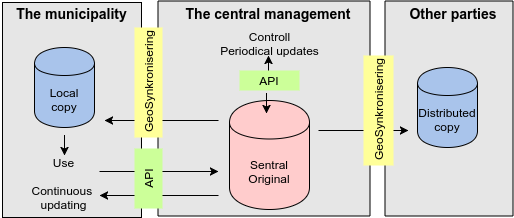
\includegraphics[scale=0.7]{img/consept.png}
%	\caption{Illustration of the concept of data distribution in the systems of both SFKB and the cadastre. The figure is adopted from \cite{Kartverket2015} }
%	\label{fig:konsept}
%\end{figure}
\begin{figure}[H]
	\centering
	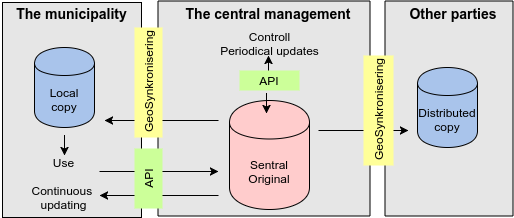
\includegraphics[scale=0.8]{img/consept.png}
	\caption{Illustration of the concept of data distribution in the systems of both SFKB and the cadastre. The figure is adapted from \cite{Kartverket2015} }
	\label{fig:konsept}
\end{figure}


%%=========================================
%\section{Plagiarism}

%\begin{quote}
%Two totally different cases, referred to as creep hypotheses $A$ and $B$, have been used as a basis of discussion to assess the effect of creep during the primary consolidation phase.
%\newline \mbox{} \hfill \citet{Deg2011Geo}
%\end{quote}
%&\end{itemize}




\chapter{Techniques for Updating and Synchronising Geodata} \label{chap:tech}
When submission of new data and modifications on existing data is done for the cadastre and basic map data in Norway, one of the criteria is that all the databases with the same content are updated regardless of where the update is done. What is needed is a geosynchronization service. The synchronization of FKB data is done with \textit{geosynchronisation}, the updating is done through the \textit{NGIS-API}, while the cadastre data is done through the \textit{MatrikkelAPIs}.  This chapter deals with these three techniques,as well as web services, for getting access to and synchronizing geospatial data.  


\section{Quadri Map Server (QMS) and Its Synchronising Services}\label{ngis}
The \textit{Quadri Map Server} (QMS) is the server of the SFKB system,
%To synchronize, update or upload data onto the QMS server, either the \textit{NGIS-API} or \textit{geosynchronisation} is used \citep{Kartverket2017}. 
and has a client-server architecture. That is, the servers distribute the data while the clients are able to both fetch and perform services on them \citep{NorkartAS2010}. 
%The NGIS-API is an application programming interface for storing spatial data, and GeoSynkronisering is a standard for synchronizing spatial data across different platforms and system solutions \citep{Kartverket2017, Kartverket2013}.
The structure of the QMS system
%with the NGIS-API
is depicted in Figure \ref{fig:qmsfig}. The \textit{archives} (data stores) are used for storing the FKB-data, the \textit{portals} define the clients and authorize users for different tasks, where a task is defined as access to an archive. The data stored in, and uploaded into, QMS is defined by the \textit{object catalogue}, and the service of translating logical, humanly meaningful, names of the distributing servers is the \textit{name server}. All the feature instances in the archives are given unique identifiers. The attributes of the identifiers are LocalId, VersionId and Namespace. Namespace is identifying the data source of the instance, the VersionId identifies the version of the object and the LocalId, based on a Universally unique identifier (UUID), ensures that each feature instance is unique\footnote{The probability to get the same number is small because there are som many possibilities. E.g., the number of random version 4 UUIDs which need to be generated in order to have a 50\% probability of at least one collision, is 2.71 quintillion. This is computed as follows: $ n \approx \frac{1}{2} + \sqrt{\frac{1}{4}+2 \times \ln{2} \times  2^{122}} \approx 2.71 \times 10^{18} $ \citep{Eggan2017}}. 
The \textit{NGIS-API} is the application programming interface for storing spatial data into QMS. \todo{skal jeg flytte denne setningen opp til over identifikatorene?}
.

\begin{figure}[H]
	\centering
	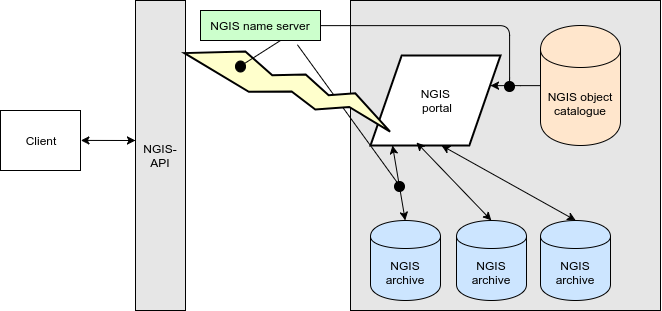
\includegraphics[scale=0.5]{img/ngiss.png}
	\caption{The structure of the Quadri Map Server (QMS) system. For updating the data in QMS the NGIS-API is used.  The main components of the system are portals, object catalogue and archives. It is possible to use geosynchronisation (chapter \ref{geosync}) to manage the data in QMS, in addition to the NGIS-API. Figure adapted from \citep{Kartverket2017b} }
	\label{fig:qmsfig}
\end{figure}

\subsection{NGIS-API}

When editing an existing object, say a building or the land use of an area, in QMS, the object gets locked in the archive, and the user edits the object locally. When the updating is done, the user has to send the object, along with objects that have been edited, added or deleted, back to its archive. When the objects are locked in the archives, other users cannot edit the same object, but they might look at it. This process is called \textit{long transactions} \citep{Kartverket2017b}.



%The service of translating logical, humanly meaningful, names of the distributing servers into unique identifiers (UUID) is the Name server. The Name server is a computer permanently connected to the Internet and is invisible to the common client of the QMS system. Because the servers are registered in the Name server at initialization, starting a server on a new machine will automatically update the Name server. 

%\subsection{Portals}
%It is the portals that handles the client access to the data in QMS, and the clients and their available tasks are defined here. A client's task is for updating and reading into QMS via teh NGIS-API

%The archives 
%\begin{itemize}
%	\item navnetjeneste
%	\item portaler
%	\item archives
%	\item object catalogues.
%\end{itemize}



\subsection{\textit{GeoSynkronisering} - the Geosynchronisation Standard}\label{geosync}

Geosynchronising (\textit{GeoSynkronisering}) is a Norwegian standard for synchronising geographical information across computer systems, and is a provider-subscriber system as illustrated in figure \ref{fig:geosync}. The \textit{provider} updates the database with new data, while the \textit{subscribers} are allowed to update their databases with the changes done by the provider. The SFKB works as a provider: if data is changed or added in QMS, the features will automaticly be geosynchronised to all subscribers. Common subscribers in the SFKB-system are the municipalities and GeoNorge. GeoNorge is the web page where public agencies and institutions, as well as private actors, can get map data and other geospatial information for Norway.  
\\
\begin{figure}[H]
	\centering
	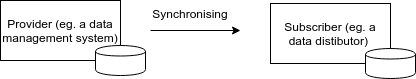
\includegraphics[scale=0.6]{img/geosync.png}
	\caption{The geosynchronisation concept, adopted from \cite[p.~16]{Kartverket2013}. }
	\label{fig:geosync}
\end{figure}


The project of making a standard interface for geosynchronisation services in Norway was carried out in 2012, and was a collaboration between Kartverket, the Norwegian Institute of Bioeconomy Research (NIBIO) and system providers in Norway. Geosynkronisering is a open and freely available project on GitHub, and this Norwegian standard is based on the concepts and methods from international standards, i.e. ISO 19100 Geographic Information/Geomatics and Open Geospatial Consortium (OGC) \citep{Eggan2017,Kartverket2013}.

The geosynchornisation standard is model driven, using models as key artefacts in the development.
%describing the data of an application or domain
UML is used on the conceptual level to describe the data, and on the the data format with GML, using XSD as an application schema showing the meta data. An example of a UML is given below.

\begin{figure}[H]
	\centering
	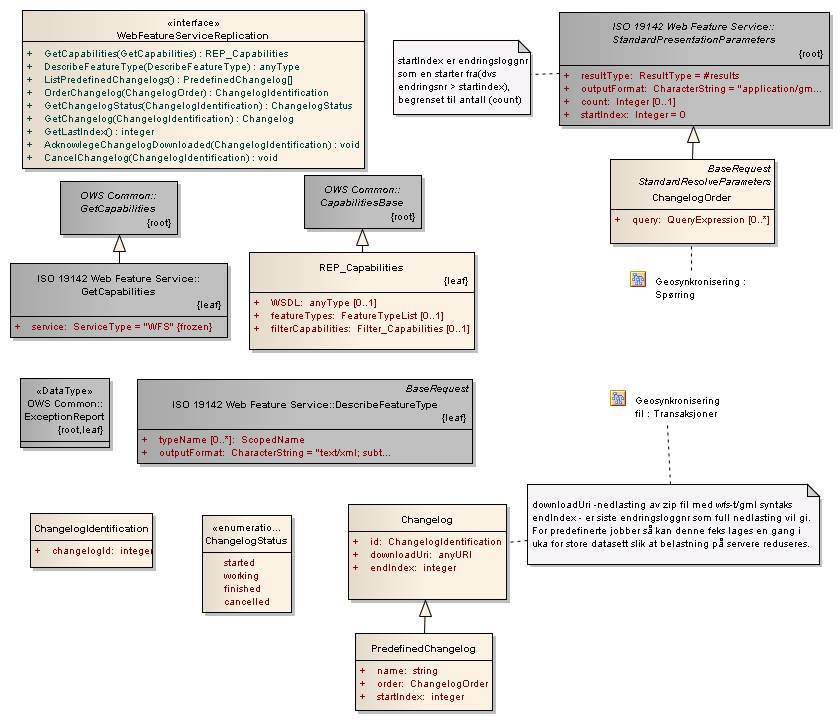
\includegraphics[scale=0.35]{img/uml.png}
	\caption{Figure from \cite{Kartverket2012a} showing an UML model of the services of the geosynchronisation.}
	\label{fig:uml}
\end{figure}

The data transfer with geosynchronising (figure \ref{fig:geosyncprocess}) is a set of transactions of changed features on the GML-format and their respective changelogs are specified by the WFS-T.  GML (Geography Markup Language) is an open interchange format for geographic transactions and a modelling language for geospatial systems \citep{OGC2017}. WFS-T (Transactional Web Feature Service) allows creation, deletion, and updating of geospatial features on the web \citep{OGCNetwork} and will be further described in chapter \ref{wfs}. 

\begin{figure}[H]
	\centering
	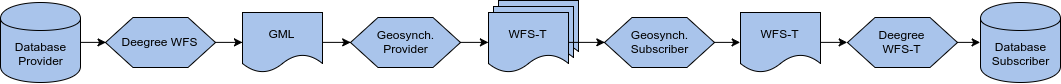
\includegraphics[scale=0.43]{img/geosynkkk.png}
	\caption{A detailed description of the Norwegian geosynchronisation process, adapted from \cite{Eggan2017}. The data stored in the database TODO . Deegree is an implementation of the Web Feature Service}
	\label{fig:geosyncprocess}
\end{figure}



%TODO Sjekk ut dette og fyll det ut: For the SFKB system the municipalities, and the other agencies managing the updating of the FKB data in Norway, will still have a local copy of the geodata. It is this copy they are editing  \citep{Kartverket2016}  
\section{The Central Cadastral Server and its APIs}
%There are several services provided by the cadastre;  The cadastral server has the logic for managing and assembling the cadastral records), as well as control and validation of the business rules of the information. Clients of the cadastre can update and read the cadastal records through the MatrikkelAPI \citep{Difi2014, Matrikkelavdelingen2017}. 
%(a further presentation of the MatrikkelAPI and system will be provided in chapter \ref{chap:matrikkelapi})
%As was stated in chapter ref 
There are several services provided by the cadastre, Matrikkelen; the \textit{cadastral server} serves all clients, both editing and viewing (figure \ref{fig:matr}). The logic of the cadastre server includes management and assembling of cadastre information, as well as control and validation of the business rules of it. The only way to get access to the data on the \textit{cadastre database} is through the \textit{MatrikkelAPI} (chapter \ref{matrikkelapi}) that is on the cadastral central server \citep[p.~338]{Matrikkelavdelingen2017}. Submissions and modifications on the cadastral data are done to the centralised data store directly, as for the new SFKB system. When wanting to keep a local cadastre copy, the Matrikkel system provides a \textit{Changelog API} for synchronizing changes on the central data store. See figure \ref{fig:matr}. 

The physical architecture of the central cadastral server is clustered, meaning there are several physical servers, but for the clients they will appear as one. %(High-Availability Cluster? \citep{IWebTechnologies2015})


\subsection{The MatrikkelAPIs} \label{matrikkelapi}
The MatrikkelAPIs is application programming interfaces for extracting data, in both small and large scale, of the cadastral data.  

There are three MatrikkelAPIs. The first one is for the clients with access to updating the cadastre data - the \textit{Editing API}, the second one the \textit{Viewer API} includes services for inspecting and reading the data and the \textit{Changelog API}, as stated earlier, provides services for fetching data changes - primarily for the local copies at the municipalities, but also for external registers.  The Viewing API support other services as well: web services as WMS that deliver georeferenced raster maps
%with addresses as points and buildings and areas for land parcels 
as well as WFS delivering vectorised map	and properties for addresses, buildings and land parcels. 

There are several types of clients to the cadastre system: the \textit{updating}-, \textit{viewing}- and \textit{retrieval clients} as well as \textit{other systems}. The updating clients support inspection and updating for all information on the cadastre, the viewing clients supports inspection of the data, as well as viewing the cadastral data joint with data from external systems, and lastly the retrieval clients supports updating external municipality registers. Other systems using the cadastre system are mainly systems that uses cadastral information for other software solutions, e.g. a municipal specialized system \citep[p.~337-338]{Matrikkelavdelingen2017}.
 
%As for the SFKB system, the municipalities updates the cadastre data directly into a national and centralized database. 

\begin{figure}[H]
	\centering
	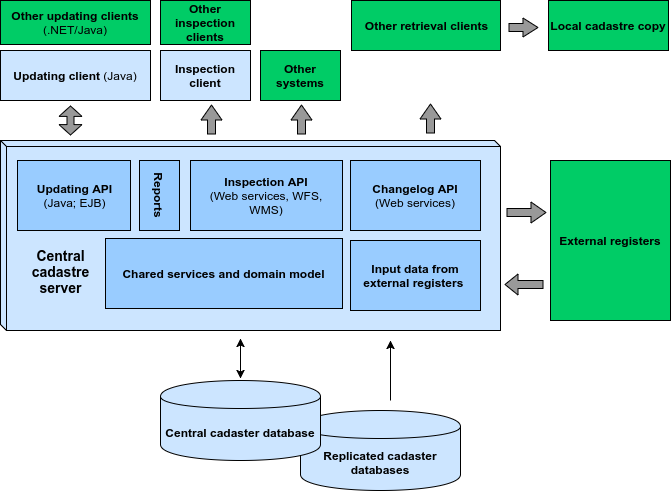
\includegraphics[scale=0.5]{img/matrikkelSYS}
	\caption{The cadastre system, \textit{Matrikkelen}. Solutions for databases through API, clients and relations to other information systems. Adapted from \citep[p.~337]{Matrikkelavdelingen2017} }
	\label{fig:matr}
\end{figure}

\section{Other Generic Services}
There are several web services, ways to access web-based geospatial data. These technologies have been created to facilitate the exchange of geospatial information and to find new ways to communicate geodata and to redefine the work flow of the geospatial analysis. In the following subchapters some of them are presented.  

\subsection{Standard Spesifications from the Open Geospatial Consortium)}\label{OGC}
To get a higher interoperability in the Geographical Information System (GIS) community the Open Geospatial Consortium (OGC) has created standard specifications for data sharing, processing, retrieval, visualisation, content and cataloguing \citep{giuliani2013}.

\subsubsection{The Web Feature Service (WFS)}\label{wfs}

The Web Feature Service (WFS) is a standard geodata extracting service for describing data manipulation on feature level \citep{Peng2005, Norgedigitalt2014}. The specification defines interfaces required to support transactions and query operations on geospatial features over the internet.

The GML-format is the defacto standard transferring format, but WFS supports other formats as well \citep{Eggan2017}. By using GML for the exhange of geospatial data,  interoperability between the heterogeneous system is provided \citep{YaoXiaobai2008Iimo}.

Whereas WFS allows queering and retrieval of features, transactional Web Feature Service (WFS-T) permits the user to create, delete and update features \citep{OGCNetwork},

\subsubsection{The Web Mapping Service (WMS)}
The Web Mapping Service (WMS) is another standad from OGS for exchanging geograpichal information over the web. When using the Web Mapping Service(WMS) the user is given an image of a map that cannot be edited or spatially analysed. 	


\subsection{Simple Object Access Protocol (SOAP)}
Simple Object Access Protocol (SOAP) is a protocol that defines how XML and HTTP are used to get access to objects, services and servers from a web based service, thus aiding in interoperability. SOAP defines an envelope for Web Service messages, where the envelope consists of a header with meta data, e.g. how the recipient of the SOAP message should interpret the message, and the body with the actual message. SOAP is often referred to as Web Service, as it is the original web service \citep{Kartverket2013}, and may serve as a standard for all systems, because it is platform independent \citep{Sipes2004}. 

The Cadastre Viewing and Changelog APIs and the geosynchonisation are examples of SOAP web services. 
%Tjenestegrensesnitt med mekanismer for å hente ut objekter fra en web-basert tjeneste. Ofte omtalt som Web Service (den opprinnelige web servicen). 


\subsection{Representational State Transfer (REST)}
The definitions of Representational State Transfer (REST) are many \citep{Fielding, Richardson}, this paper uses the description by \cite{Fieldinga}: \textit{REST is a coordinated set of architectural constraints that attempts to minimize latency and network communication while at the same time maximizing the independence and scalability of component implementations}. 
%\cite{Battle2008}: \textit{REST is a pattern of resource operations that has emerged as a de facto standard for service design in Web 2.0 applications.} 

REST is commonly based on the HTTP and HTML standards, and provide simplified calls to services through HTTP. It is only data structures and the transferring of their state that is dealt with in a RESTful service \cite{Battle2008}. The state transferring calls are POST, GET, PUT and DELETE, which receptively creates, reads, updates and deletes resources in the RESTful service. A resource is identified and resolved with a URL.

\begin{figure}[H]
	\centering
	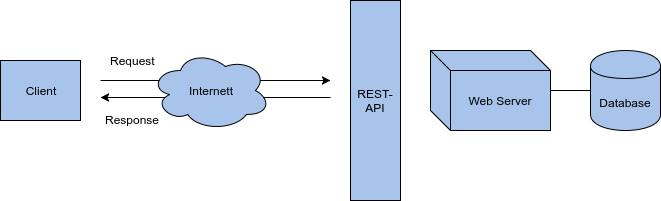
\includegraphics[scale=0.5]{img/REST}
	\caption{REST-API: Clients use  HTTP (or other protocols') queries to create, read, update and delete data on the server-side applications.  Adapted from \citep{Ceeb2013} }
	\label{fig:rest}
\end{figure}

%Representational State Transfer. En tilleggsmekanisme til HTTP som forenkler kall mot tjenester via HTTP. 



\chapter{Equivalent systems in the other Scandinavian countries}
 As each country normally operates with separate file formats for the geospatial data \cite{Frenvik2017}
 Infrastructure for Spatial Information in the European Community (INSPIRE) is the European collaboration for a common standards for describing and sharing spatial data \cite{INSPIRE}. In the following sections there will be brief explanations of the geodata systems in Sweden and Denmark.


\section{Sweden}
The mapping authority in Sweden is Lantm\"{a}teriet. Lantm\"{a}teriet grant maps, aerial images and other geographical information about Sweden, together with central and local authorities. Students, scientist or employees of universities or other educational and cultural institutions can get the geodata provided by the Lantm\"{a}teriet for free. \todo{https://www.lantmateriet.se/en/Maps-and-geographic-information/} 

\subsection{The geodata cooperation, \textit{Geodatasamverkan}  evt geodataportalen} \todo{https://www.geodata.se/anvanda/geodatasamverkan/}

 
geodatas

\section{Denmark}
Geodatastyrelsen "Kartverket" http://gst.dk/om-os/
Datafordeleren http://sdfe.dk/hent-data/datafordeleren/
Grunndataprogrammet Sara Bjerre på sarbj@digst.dk
Matrikkelen http://gst.dk/matriklen/ejendomsdataprogrammet/matriklens-udvidelse/



\subsection{INSPIRE}

\chapter{Directly Updating versus Local Updating}
The benefits of the new SFKB sytem are numerous, as compared to local storage; freshly updated data for the end-users of map data, and the changes will carry through to \textit{all} end-users, as opposed to local storage, which only applies to the users of that specific municipality (blir det riktig å anta at kommunene distribuerer fra sin lokale kopi mens de har de dataene?) \citep{Dontigney2017}. Another benefit is a more efficient and effective validation process, as the requirements are defined and validated one place and every change to the central store is done by the agency where the change actually occurred \citep{Kartverket2017e}. 

There are several(TODO: siter flere) authors that agrees on the benefits, the Canadian geosynchronisation project was according to \cite{Reichardt2012} providing the most current and reliable data, consequently avoiding unnecessary versioning and keeping the duplication of data at a minimized level. As the Norwegian geosynchronisation standard is based on the same standards as the Canadian - \cite[p.~7]{Kartverket2013}  TODO: KILDE!! Stemmer det??


%Centralisation of data management within different scientific fields where sharing and analysing data is major tasks have been important for (...), and entering data directly into databases     In the paper \textit{A Generic framework for synchronidistributed data management in archaeological related disiplines} \cite{LOHRER2016558} discuss the advantages and disadvantages of centralised data management within the archaeological field

\subsubsection{Spatial Data Infrastuctures}

According to \cite{Peng2005} sharing data on file level is causing latency in update of the data, and it is difficult to deduce a generalised standardisation for all geodata, and reaching consensus might be difficult.  Spatial data infrastructure (SDI) seek to facilitate the access and integration of geospatial data coming from various sources. To achieve this objective, systems must be interoperable. \cite{giuliani2013} 

With the standard for exchanging geospatial data in Norway, SOSI (Samordnet Opplegg for Stedfestet Informasjon) (...) /   
One of the disadvantages of updating directly into a data store is that, as was stated earlier in this chapter, that it may be difficult to obtain a generalised data format and that validation thus will be difficult. As the Norwegian geospatial data have been standardised through the SOSI-standardisation for 30 years this will not be a problem (formuler annerledes). Validation problems wil mainly be because of humanly errors.    (TODO: finne kilder som argumenterer for at valideringsprossessen blir lettere, eller er dette et diskusjonskapittel? ) 

%The SOSI format can be a quite touchy subject in the Norwegian geomatic's community. 

%The SOSI-format and the SOSI-standard 
%In Norway there is a standard for exchanging geospatial data: SOSI (Samordnet Opplegg for Stedfestet Informasjon). When mentioning SOSI it is hard not to 


%SOSI – Samordnet Opplegg for Stedfestet Informasjon. SOSI har hittil vært kjent som et format, men er mye mer. Standardene utarbeides som UML-modeller, og kan representeres ved ulike formater. SOSI er nå i en overgangsfase mellom SOSI prikkformat og SOSI GML-format. SOSI følger de internasjonale standardiseringsarbeidet i OGC og ISO/TC 211, samt INSPIRE.

%GML – Geographic Markup Language GML er et «rikt» format og står for Geographic Markup Language, og er basert på XML. Kartverket har lagt ned mye jobb i å gå fra SOSI prikkformat til GML-format. Det arbeides med mulighet for å levere FKB-data og arealplan-data på GML. Se Link: https://en.wikipedia.org/wiki/Geography_Markup_Language

%SOSI prikkformat: Det formatet som hittil har vært dominerende og godt kjent i Norge, men er tenkt erstattet av GML. SOSI prikkformat er et «rikt» format, men GML er «rikere». Det er vedtatt ikke å utvide det sær-norske SOSI prikkformatet og heller ta i bruk GML.





%Perhaps not as a seperate chaper, but as a part of the introduction?
%\begin{itemize}
%	\item definitions of centralized and decentralized system
%	\item pros and cons
%	\item Kartverket's web page of QA 
%	\item check reference list: \url{https://en.wikipedia.org/wiki/Centralized_database} 
%\end{itemize}

%"Centralized database storage, although it sometimes limits responsiveness to individual users, offers a number of key advantages for businesses."  \cite{Dontigney2017}

%"Centralized storage requires the business to invest heavily in the server technology, such as fault tolerance, but also allows it to cut overall costs. The maintenance to the central server proves less costly than maintenance to multiple computers, especially if the business operates in multiple locations. Centralized storage also reduces overall space requirements for data storage and processing.

%... improved reliability and update speed: Updates carried out on a database run on centralized storage carry through to all end-users, as opposed to local storage, which only applies to that computer. " \cite{Dontigney2017}



%Previous work - storing centrally

%\cite{Breslow2004}

%"Add to this the fact that file sizes and data storage requirements are increasing year after year, and the efficient sharing of files across distributed enterprises over the wide area network (WAN) has become a Herculean task.

%The problem is that although gigabytes of data can easily be shared over a local area network (LAN) using standard file server technology, they cannot so easily be shared across remote offices connected over the WAN. In truth, standard file server protocols provide unacceptably slow response times while opening and writing files over the WAN and this forces remote office IT managers to make some unappealing choices. IT managers and network users must either live with reduced productivity due to poor network performance at remote offices or they must use replication schemes that waste storage and inhibit global collaboration."




\begin{itemize}
	\item \cite{Breslow2004} WAN
	\item coherency - garantert aldri konflikt med adre oppdateringer
	\item consistency - dataene er up-to-date
\end{itemize}
%"Data coherency and data consistency are important properties of WAFS implementations, because they ensure that file updates are safe (cannot be written over) and available throughout the network of edge devices-crucial features for supporting engineering collaboration.

%Data coherency means that file updates (writes) from any one remote office are guaranteed never to conflict with updates from antrther remote office. Properly designed WAFS implementations guarantee this by maintaining a system of file leases. Leases are defined as a particular access privilege to a file from a remote office.

%...
%Data consistency implies that file updates made at one office are always available enterprise-wide, and well-architected WAFS system do this immediately after the update is made. Again, for collaboration, this is supremely important because remote designers want to be sure they are working on the most current version of any file, no matter where it was worked on last."


%Dette er utenfor scopet: 
%Taking a broader look at the concept of centralising, there are some fields that do not encourage centralising network infrastructures. Such as within the field of waste water management, electricity  and heater and water supply \cite{Eggimann2016}. 







\subsection{Previous work - generic API's}
This chapter will present papers concerning generic API's and framwork depending API's

%Bruk og argumenter for/mot bruk av generiske tjenester (WMS, WFS, WPS), kontra egne spesialiserte API'er (?). Plattformuavhengige API'er (WebService, REST) vs. plattformavhengigeAPI'er.

\cite{giuliani2013} wanted in their paper to benchmark and evaluate the quality of the web services WFS and WCS (Web Coverage Service). They conclude that, amongst other things, the OGC specifications (WFS, WCS) are providing interoperable access to data in an efficient and timely manner, and that the specifications are not convenient for transferring large volumes of data. 

----Kan jeg rerferere til samtale?-----
- zipped GML da gjør det ikke noe at det er store filer, smat større datamaskiner



%Although the promise of SOAP (and Web services) is portability, reality often bites back with a vengeance. Even our example application requires care and experimentation to make exception handling work across different SOAP implementations. Other quirks (for instance, handling the soapAction attribute in line 51 of the WSDL) can provide hours of frustration. It’s always good to keep in mind that communicating with XML can be very inefficient. Because XML is textual and verbose, converting data to XML and back can hog application performance. On the other hand, in distributed applications over the network, factors such as network latency are likely to be just as important. Still, the fact that technology now lets us build interoperable, distributed applications doesn’t mean that all the applications we build from now on will be of that ilk. As always, a careful assessment of the specific requirements is essential, before rushed decisions

%Because GML, SVG, WFS, and WMS are all international industry standards, the greatest strength of the proposed framework lies in the promised syntactic interoperability. \cite{YaoXiaobai2008Iimo}


%Several studies [8,13,21] have shown that projects that have adopted and implemented geospatial interoperability standards saved around 25 percent of their time, compared to those who rely on proprietary standards. These reports also showed that using geospatial interoperability standards lowers the transaction costs for sharing data and information. The fact that exchange of data and information is performed on standardized interfaces enhances flexibility and adaptability of projects over time. \cite{giuliani2013}

\chapter{Conclusion}

\begin{itemize}
	\item Matrikkelen har fungert fint til nå
	\item oppsummere noe fra litterature review
	\item version-control issues as well as inefficient collaboration for storing local copies
	\item keeping service databases up-to-date in a multi-provider situation. %https://www.maanmittauslaitos.fi/sites/maanmittauslaitos.fi/files/attachments/2017/09/geoprocessing_2015_1_20_30079.pdf
	
\end{itemize}


%Fordel:
%---

%Ulempe:
%"A third key business objective was to address the increasing customer demands for improved application availability, not only in terms of failure recovery, but for the more important reduction of planned outage times. Today, there is less opportunity for planned systems shutdowns in the global economic environment. Here again, meeting this objective was key to the Parallel Sysplex cluster design." \cite{Nick1997}

%"Terry Walby, datacentre solutions director at Computacenter Services, warned that centralisation was putting huge pressure on power supplies and space in the datacentre. To mitigate the problems caused, Walby said server virtualisation was being explored by many firms, and storage virtualisation was also being taken more seriously." \cite{Tash2006}


%\cite{doi:10.1080/17538947.2017.1351583}   A paradigm-shift is needed, not only on the side of data providers, but also on the side of users who use large volumes of geospatial data. Data users have to shift from the traditional geospatial data workflow where large volumes of data have been downloaded and replicated onto local machines towards a workflow with integrated web service standards for data access and processing, that does not require time-consuming data download anymore. Data providers have to be more progressive towards offering server-based data access and processing in a standardised and interoperable way.


%Because GML, SVG, WFS, and WMS are all international industry standards, the greatest strength of the proposed framework lies in the promised syntactic interoperability. \cite{YaoXiaobai2008Iimo}


%As this paper has presented there are a few drawbacks of updating directly to a central data store. On the other hand, the benefits seem to be greater, and thus the SFKB-system have a bright future ahead; providing a greater national collaboration of the basic map data, where the end-users may rest assured of fresh data of high quality.


%Further investigated 
%Future work : This includes tracking latencies, bottlenecks, and errors that may negatively influence its overall quality. \cite{giuliani2013}

The process of storing map data locally and later send those data to \textit{Kartverket} was perhaps unnecessarily time-consuming and inefficient. As this paper has presented there are a few drawbacks of updating directly to a central data store. On the other hand, the benefits seem to be greater and thus the SFKB-system seems to have a bright future ahead; the \textit{SFKB}-system will reduce operational cost by lessening the import, export, copying and control costs of the data, as \cite{Kartverket2017e} sums it up.  This is in addition to improving service delivery for the public, providing it with fundamental and reliable map data freshly updated at all times. 

% Include more chapters as required.
%%=========================================
\appendix
%This is Appendix A - Acronyms
%%=========================================

\chapter{Glossary}\label{glossary}
\begin{description}
	\item[API] Application Programming Interface
	\item[FKB] Felles kartdatabase (The basic map data)
	\item[GML] 
	\item[INSPIRE] Infrastructure for Spatial Information in the European Community (An European collaboration for a common geographical infrastructure)
	\item[UUID] Universally Unique Identifier (A number used to identify objects, all feature instances in SFKB have a LocalId based on an UUID)
	\item[Matrikkelen] The Cadastre
	\item[OGC] Open Geospatial Consortium
	\item[NGIS] API for updating features saved in QMS
	\item[QMS] Quadri Map Server (The server for the SFKB system)
	\item[REST] Representational State Transfer 
	\item[SDI] Spatial Data Infrastuctures
	\item[SOAP] Simple Object Access Protocol
	\item[SOSI] Samordnet Opplegg for Stedfestet Informasjon
	\item[SFKB] Sentral Felles kartdatabase (The Central Map Data Store)
	\item[UML] Unified Modeling Language
	\item[WCS] Web Coverage Service
	\item[WFS] Web Feature Service
	\item[WFS-T] Web Feature Service Transactional
	\item[WMS] Web Map Service
\end{description}

%This is an Appendix
%%=========================================

\chapter{Additional Information}
This is an example of an Appendix. You can write an Appendix in the same way as a chapter, with sections, subsections, and so on.

%%=========================================
\section{Introduction}

%%=========================================
\subsection{More Details}
% Include more appendices as required.
%%=========================================
%\bibliographystyle{apa}
\addcontentsline{toc}{chapter}{\bibname}
\bibliography{bibtex/library}  
%%=============================================
%\glsaddall %Adding all glossary entries
\end{document}
